\chapter{Généralités sur les fonctions}

\section{Généralités}

\subsection{Image et antécédents}

\def\manote{Le concept de fonction s'est construit progressivement au XVII\textsuperscript{e} siècle avec les travaux de \textbf{René Descartes} et \textbf{Pierre de Fermat}, qui ont révolutionné les mathématiques en reliant la géométrie aux équations algébriques via le système de coordonnées. Cependant, c'est au XVIII\textsuperscript{e} siècle que \textbf{Leonhard Euler} a formalisé la notion moderne, définissant la fonction comme une relation analytique précise permettant de lier deux variables entre elles.}

\definition [Fonction numérique\sidenote{\manote} - image]

Étant donné $I$ un intervalle de $\R$, une \textbf{fonction numérique} $f$ définie sur $I$ est une relation qui à tout $x$ de $I$ associe un \textbf{unique} réel, noté $f(x)$ et appelé \textbf{image} de $x$ par $f$.

\rem

Notations possibles :

\begin{itemize}
	\item $f$ est la fonction définie sur $I$ par $f(x)=\cdots$
	\item $\begin{array}{rcl}f : I& \to& \R\\ x &\mapsto &f(x)=\cdots\end{array}$
\end{itemize}

\ex\sidenote{Nous pouvons utiliser une calculatrice en mode tableur pour automatiser les calculs\\ \cimg{\linewidth}{img/fct/calc.png}}

Soit $f$ la fonction définie sur $\R$ par $f(x)=2x^2+3$.

\begin{itemize}
	\item L'image de $0$ par $f$ est $f(0)=2\times 0^{2}+3=3$.
	\item L'image de $1$ par $f$ est $f(1)=2\times 1^{2}+3=5$.
	\item \ldots
	      % \item Pour tous réels $a$ et $b$ : $f(b)-f(a)=(2b^{2}+3)-(2a^{2}+3)=2b^{2}-2a^{2}=2(b^{2}-a^{2})$.
\end{itemize}

\definition [Antécédents]

Étant donné une fonction $f$ définie sur $I$.

Pour tout réel $b$, on appelle \textbf{antécédents} de $b$ par $f$ tous les réels $x$ de $I$ (s'ils existent) tels que $f(x)=b$.

\ex

Soit $f$ la fonction définie sur $\R$ par $f(x)=x^2+1$.
\begin{itemize}
	\item \textit{Antécédents de $1$} :\\ \ms
	      $$\def\arraystretch{1.5}
		      \begin{array}{rl}
			      ~    & f(x)=1                                    \\
			      \iff & x^{2}+1=1 \quad \iff x^2=0 \quad \iff x=0
		      \end{array}
	      $$
	      $0$ est le seul antécédent de $1$ par $f$.
	      \newpage
	\item \textit{Antécédents de $5$} :\\ \ms
	      $$\def\arraystretch{1.5}
		      \begin{array}{rl}
			      ~    & f(x)=5                                                     \\
			      \iff & x^{2}+1=5\quad \iff x^2=4\quad \iff x=2\,\text{ ou }\,x=-2
		      \end{array}
	      $$
	      $2$ et $-2$ sont les deux antécédents de $5$ par $f$.

	\item \textit{Antécédents de $0$} :\\ \ms
	      $$\def\arraystretch{1.5}
		      \begin{array}{rl}
			      ~    & f(x)=0                                                         \\
			      \iff & x^{2}+1=0 \quad \iff x^2=-1\quad \text{(impossible dans $\R$)}
		      \end{array}
	      $$
	      $0$ n'admet aucun antécédent par $f$.
\end{itemize}

\subsection{Courbe représentative d'une fonction}

\definition [Courbe représentative]

\def\manote{~\\ \begin{tikzpicture}
		\draw[->, >=Triangle, line width=1pt] (-0.5,0) -- (3.5,0) node[right] {$x$};
		\draw[->, >=Triangle, line width=1pt] (0,-0.5) -- (0,3.5) node[above] {$y$};
		\draw[domain=0:3, smooth, variable=\x, blue, line width=1.5pt] plot ({\x}, {0.5*\x*\x/2 + 0.5});
		\draw[dashed] (2,0) -- (2,1.5);
		\draw[dashed] (0,1.5) -- (2,1.5);
		\node[below, font=\large] at (2,-0.1) {$x$};
		\node[left, font=\large] at (0,1.5) {$f(x)$};
		\node[above right,font=\large] at (2.3,2.5) {$\Cf$};
		\fill[red] (2,1.5) circle (2pt);
	\end{tikzpicture}}

Dans un repère $(O,\vec{i},\vec{j})$, on appelle \textbf{courbe représentative}\sidenote{\manote} de la fonction $f$ définie sur $I$ l'ensemble des points d'abscisse $x$ et d'ordonnée $f(x)$ pour tous les $x$ de $I$.

\rem

Notation courante : $\mathcal{C}_{f}$.

Une équation de la courbe est $y=f(x)$.

\prop

\begin{itemize}
	\item \textbf{Lecture graphique de l'image} d'un réel $a$ par $f$\\ On repère le point de $\Cf$ d'abscisse $a$ et on lit son ordonnée $f(a)$.\\
	      \begin{center}
		      \begin{tikzpicture}
			      \draw[->, >=Triangle, line width=1pt] (-0.5,0) -- (3.5,0) node[right] {$x$};
			      \draw[->, >=Triangle, line width=1pt] (0,-0.5) -- (0,3.5) node[above] {$y$};
			      \draw[domain=0:3.3, smooth, variable=\x, blue, line width=1.5pt] plot ({\x}, {-0.5*\x*\x/4 + 2});
			      \def\a{2}\def\fa{1.5}
			      \draw[->, >=Triangle, thick] (\a,0) -- (\a,\fa);
			      \draw[->, >=Triangle, thick] (\a,\fa) -- (0,\fa);
			      \node[below, font=\large] at (\a, -0.1) {$a$};
			      \node[left, font=\large] at (0,\fa) {$f(a)$};
			      \node[above right,font=\large] at (3,0.7) {$\Cf$};
			      \fill[red] (\a,\fa) circle (2pt);
		      \end{tikzpicture}
	      \end{center}

	\item \textbf{Lecture graphique des antécédents} d'un réel $b$ par $f$\\ On repère les points de $\Cf$ d'ordonnée $b$ et on lit leurs abscisses.

	      \begin{center}
		      \begin{tikzpicture}
			      \draw[->, >=Triangle, line width=1pt] (-0.5,0) -- (3.5,0) node[right] {$x$};
			      \draw[->, >=Triangle, line width=1pt] (0,-0.5) -- (0,3.5) node[above] {$y$};
			      \draw[domain=0:3.3, smooth, variable=\x, blue, line width=1.5pt] plot ({\x}, {0.3125*(\x-1.6)*(\x-1.6)+1});
			      \def\b{1.2}
			      \draw[dashed] (0,\b) -- (3.2,\b);
			      \def\xA{0.8}\def\xB{2.4}
			      \draw[->, >=Triangle, thick] (\xA,\b) -- (\xA,0);
			      \draw[->, >=Triangle, thick] (\xB,\b) -- (\xB,0);
			      \node[left, font=\large] at (0,\b) {$b$};
			      \node[below, font=\large] at (\xA,-0.1) {$x_1$};
			      \node[below, font=\large] at (\xB,-0.1) {$x_2$};
			      \node[above right,font=\large] at (3,1.9) {$\Cf$};
			      \fill[red] (\xA,\b) circle (2pt);
			      \fill[red] (\xB,\b) circle (2pt);
		      \end{tikzpicture}
	      \end{center}

\end{itemize}

\section{Sens de variation d'une fonction sur un intervalle}

\definition [Fonctions croissante et décroissante]

\begin{itemize}
	\item Une fonction $f$ est dite \textbf{croissante} sur un intervalle $I$ si, pour \textbf{tous} les réels $a$ et $b$ de $I$ tels que $a<b$, on a $f(a)\le f(b)$.\sidenote{Les images sont rangées dans le même ordre que les antécédents.}
	\item Une fonction $f$ est dite \textbf{décroissante} sur un intervalle $I$ si, pour \textbf{tous} les réels $a$ et $b$ de $I$ tels que $a<b$, on a $f(a)\ge f(b)$.\sidenote{Les images sont rangées dans l'ordre contraire de celui des antécédents.}
\end{itemize}

\begin{center}
	\begin{tikzpicture}[scale=1, >=Triangle]
		\begin{scope}
			\draw[->] (-0.5,0) -- (4,0) node[right, font=\small] {$x$};
			\draw[->] (0,-0.5) -- (0,4) node[above, font=\small] {$y$};
			\def\xa{0.8} \def\ya{0.75}
			\def\xb{3.2} \def\yb{2.55}
			\draw[thick, black, domain=0.2:3.8] plot (\x, {0.15*(\x+0.5)^2 + 0.5});
			\draw[dashed, gray] (\xa,0) node[below, black, font=\small] {$a$} -- (\xa,\ya) -- (0,\ya) node[left, black, font=\small] {$f(a)$};
			\draw[dashed, gray] (\xb,0) node[below, black, font=\small] {$b$} -- (\xb,\yb) -- (0,\yb) node[left, black, font=\small] {$f(b)$};
			\node[circle, fill=blue, inner sep=1.5pt, label={[blue]above :$A$}] at (\xa,\ya) {};
			\node[circle, fill=blue, inner sep=1.5pt, label={[blue]above :$B$}] at (\xb,\yb) {};
		\end{scope}
		\begin{scope}[xshift=6cm]
			\draw[->] (-0.5,0) -- (4,0) node[right, font=\small] {$x$};
			\draw[->] (0,-0.5) -- (0,4) node[above, font=\small] {$y$};
			\def\xa{0.8} \def\ya{3.25}
			\def\xb{3.2} \def\yb{1.45}
			\draw[thick, black, domain=0.2:3.8] plot (\x, {-0.15*(\x+0.5)^2 + 3.5});
			\draw[dashed, gray] (\xa,0) node[below, black, font=\small] {$a$} -- (\xa,\ya) -- (0,\ya) node[left, black, font=\small] {$f(a)$};
			\draw[dashed, gray] (\xb,0) node[below, black, font=\small] {$b$} -- (\xb,\yb) -- (0,\yb) node[left, black, font=\small] {$f(b)$};
			\node[circle, fill=blue, inner sep=1.5pt, label={[blue]above :$A$}] at (\xa,\ya) {};
			\node[circle, fill=blue, inner sep=1.5pt, label={[blue]above :$B$}] at (\xb,\yb) {};
		\end{scope}
	\end{tikzpicture}
\end{center}

\rem
\begin{itemize}
	\item En remplaçant $f(a)\le f(b)$ par $f(a)<f(b)$, on dit que $f$ est \textbf{strictement croissante} sur $I$.
	\item En remplaçant $f(a)\ge f(b)$ par $f(a)>f(b)$, on dit que $f$ est \textbf{strictement décroissante} sur $I$.
	\item Quand une fonction est croissante ou décroissante sur un intervalle, on dit qu'elle est \textbf{monotone} sur cet intervalle.
\end{itemize}

\methode [Étudier le sens de variation de $f$ sur $I$]
\begin{enumerate}
	\item On considère deux réels $a$ et $b$ quelconques dans $I$ tels que $b-a>0$.
	\item On calcule $f(b)-f(a)$ en factorisant le résultat si possible.
	\item On étudie le signe de $f(b)-f(a)$ :
	      \begin{itemize}
		      \item si $f(b)-f(a)$ reste positif sur $I$, alors $f$ est \textbf{croissante} sur $I$ ;
		      \item si $f(b)-f(a)$ reste négatif sur $I$, alors $f$ est \textbf{décroissante} sur $I$.
	      \end{itemize}
\end{enumerate}

\ex\sidenote{Représentation de $f(x)=3x^2$\begin{center}\begin{tikzpicture}[xscale=1.7]
			\draw[->, >=Triangle, line width=1pt] (-1.2,0) -- (1.2,0) node[right] {$x$};
			\draw[->, >=Triangle, line width=1pt] (0,-0.5) -- (0,3.5) node[above] {$y$};
			\draw[domain=-1.05:1.05, smooth, variable=\x, blue, line width=1.5pt] plot ({\x}, {3*\x*\x});
			\node[below left] at (0,0) {$O$};
			\node[below left,font=\large] at (1,3.4) {$\Cf$};
		\end{tikzpicture}\end{center}
}

Soit $f$ la fonction définie sur $\R$ par $f(x)=3x^2$.

\begin{itemize}
	\item \textit{Sens de variation sur $\intoo{-\infty}{0}$} :\\
	      Pour tous $a,b\in\intoo{-\infty}{0}$ avec $b-a>0$ :
	      $$\def\arraystretch{1.5}
		      \begin{array}{rl}
			      f(b)-f(a) & =3b^{2}-3a^{2} \\
			                & =3(b-a)(b+a)
		      \end{array}
	      $$
	      Or : \bi\item $b-a>0$\item  $b+a<0$ (car $a<0$ et $b<0$)\ei
	      Donc $f(b)-f(a)<0\implies f$ est \textbf{décroissante} sur $\intoo{-\infty}{0}$.

	\item \textit{Sens de variation sur $\intoo{0}{+\infty}$} :\\
	      Pour tous $a,b\in\intoo{0}{+\infty}$ avec $b-a>0$ :
	      $$\def\arraystretch{1.5}
		      \begin{array}{rl}
			      f(b)-f(a)=3(b-a)(b+a)
		      \end{array}
	      $$
	      Or : \bi\item $b-a>0$\item $b+a>0$ (car $a>0$ et $b>0$)\ei
	      Donc $f(b)-f(a)>0\implies f$ est \textbf{croissante} sur $\intoo{0}{+\infty}$.
\end{itemize}

\prop [Tableau de variations]

Le \textbf{tableau de variations} d'une fonction permet de résumer :
\begin{itemize}
	\item les intervalles sur lesquels la fonction est croissante ou décroissante ;
	\item les valeurs importantes de la fonction.
\end{itemize}

\medskip

\textbf{Lecture :}
\begin{itemize}
	\item une flèche montante signifie que la fonction est croissante ;
	\item une flèche descendante signifie que la fonction est décroissante.
\end{itemize}

\ex [$f(x)=3x^2$]

\begin{center}
	\begin{tikzpicture}[thick]
		\tkzTabInit[lgt=2.5,espcl=2.5]{$x$/1,$f(x)=3x^2$/1.5}
		{$-\infty$, $0$, $+\infty$}
		\tkzTabVar{+/$+\infty$,-/$0$,+/$+\infty$}
	\end{tikzpicture}
\end{center}


\subsection{Maximum et minimum d'une fonction sur un intervalle}

\definition [Maximum et minimum]

Étant donné $f$ une fonction définie sur $\intff{a}{b}$ contenant $x_0$ :
\begin{itemize}
	\item $f$ admet un \textbf{mini.} en $x_0$ sur $\intff{a}{b}$ si pour tout $x\in\intff{a}{b}$, on a : $$f(x)\ge f(x_0)$$
	\item $f$ admet un \textbf{maxi.} en $x_0$ sur $\intff{a}{b}$ si pour tout $x\in\intff{a}{b}$, on a : $$f(x)\le f(x_0)$$
\end{itemize}

\begin{fullwidth}
	\begin{center}
		\begin{tikzpicture}[scale=1.3, >=Triangle]
			\begin{scope}
				\draw[->] (-0.5,0) -- (4.5,0) node[right, font=\small] {$x$};
				\draw[->] (0,-0.5) -- (0,3) node[above, font=\small] {$y$};
				\draw[thick, black, domain=0.3:4] plot (\x,{0.45*(\x-2)^2+0.7});
				\draw[dashed, black] (0.6,0) node[below] {$a$} -- (0.6,1.6);
				\draw[dashed, black] (3.4,0) node[below] {$b$} -- (3.4,1.6);
				\draw[dashed, gray] (2,0) node[below, black] {$x_0$} -- (2,0.7) -- (0,0.7) node[left, black] {$f(x_0)$};
				\node at (2,-0.8) {\small Minimum de $f$};
				\fill[blue] (2,0.7) circle (2pt);
				\fill[blue] (0.6,1.6) circle (2pt);
				\fill[blue] (3.4,1.6) circle (2pt);
			\end{scope}
			\begin{scope}[xshift=6cm]
				\draw[->] (-0.5,0) -- (4.5,0) node[right, font=\small] {$x$};
				\draw[->] (0,-0.5) -- (0,3) node[above, font=\small] {$y$};
				\draw[thick, black, domain=0.3:4] plot (\x,{-0.45*(\x-2)^2+2.2});
				\draw[dashed, black] (0.6,0) node[below] {$a$} -- (0.6,1.3);
				\draw[dashed, black] (3.4,0) node[below] {$b$} -- (3.4,1.3);
				\draw[dashed, gray] (2,0) node[below, black] {$x_0$} -- (2,2.2) -- (0,2.2) node[left,black] {$f(x_0)$};
				\fill[blue] (0.6,1.3) circle (2pt);
				\fill[blue] (3.4,1.3) circle (2pt);
				\fill[blue] (2,2.2) circle (2pt);
				\node at (2,-0.8) {\small Maximum de $f$};
			\end{scope}
		\end{tikzpicture}
	\end{center}
\end{fullwidth}

\ex

\def\manote{\null\\
	\begin{tikzpicture}[scale=0.6, >=Triangle]
		\draw[->] (-5.8,0) -- (4,0) node[right] {$x$};
		\draw[->] (0,-2.8) -- (0,4.8) node[above] {$y$};
		\draw[thick, blue, domain=-5:-2, samples=10] plot (\x, {0.33*\x*\x + 1.33*\x + 2.33});
		\draw[thick, blue, domain=-2:0, samples=10] plot (\x, {0.5*\x*\x + 2*\x + 3});
		\draw[thick, blue, domain=0:3, samples=10] plot (\x, {0.09*\x*\x*\x - 0.63*\x*\x - 0.62*\x + 3});
		\draw[dashed, gray] (-5,0) |- (0,4);  % f(-5)=4
		\draw[dashed, gray] (-2,0) |- (0,1);  % f(-2)=1
		\draw[dashed, gray] (3,0)  |- (0,-2); % f(3)=-2
		\draw[dashed, gray] (2,0)  -- (2,0.1); % Pour marquer l'antécédent 2
		\fill (-5,4)  circle (3pt); % Max global (-5,4)
		\fill (-2,1)  circle (3pt); % Min local (-2,1)
		\fill (0,3)   circle (3pt); % Max local (0,3)
		\fill (2,0)   circle (3pt); % Antécédent de 0 est 2 (f(2) = 0.04 ≈ 0)
		\fill (3,-2)  circle (3pt); % Min global (3,-2)
		\node[below] at (-5,0) {$-5$};
		\node[below] at (-2,0) {$-2$};
		\node[below left] at (0,0) {$0$};
		\node[below] at (2,0) {$2$};
		\node[above] at (3,0) {$3$};
		\node[right] at (0,4) {$4$};
		\node[right] at (0,3) {$3$};
		\node[right] at (0,1) {$1$};
		\node[left]  at (0,-2) {$-2$};
		\node[blue, above right] at (-4,2.5) {$\mathcal{C}_f$};
	\end{tikzpicture}
}

Une fonction $f$ est définie sur $\intff{-5}{3}$ par sa courbe\sidenote{\manote}. On peut lire :

\begin{itemize}
	\item $f(-2)=1$.
	\item L'antécédent de $0$ est $2$.
	\item $f$ admet un minimum sur $[-5\,;\,0]$ en $x=-2$.
	\item $f$ admet un minimum sur $[-5\,;\,3]$ en $x=3$.
	\item $f$ admet un maximum sur $[-2\,;\,2]$ en $x=0$.
	\item $f$ admet un maximum sur $[-5\,;\,3]$ en $x=-5$.
\end{itemize}

\section{Résolution graphique d'équations et d'inéquations}

\prop

Étant donné une fonction $f$ définie sur $I$ et $\Cf$ sa courbe représentative.
\begin{itemize}
	\item Les solutions sur $I$ de l'équation $f(x)=mx+p$ sont les \textbf{abscisses des points d'intersection} entre $\Cf$ et la droite $d$ d'équation $y=mx+p$.
	      \begin{itemize}
		      \item Cas particulier : les solutions de $f(x)=0$ sont les abscisses des points d'intersection entre $\Cf$ et \textbf{l'axe des abscisses}.
	      \end{itemize}
	\item Les solutions de $f(x)\ge mx+p$ sont les abscisses des points de $\Cf$ situés \textbf{au-dessus ou sur} la droite $d$.
	\item Les solutions de $f(x)\le mx+p$ sont les abscisses des points de $\Cf$ situés \textbf{en-dessous ou sur} la droite $d$.
\end{itemize}

\begin{fullwidth}
	\begin{center}
		\begin{tikzpicture}[scale=1.3,y=0.5cm,x=1cm]
			\draw[->,>= Triangle] (-1,0) -- (6,0) node[right] {$x$};
			\draw[->,>= Triangle] (0,-2) -- (0,8) node[above] {$y$};
			\draw[thick,blue,domain=0:5,smooth] plot (\x,{1.2*(\x-1)*(\x-4)+1}) node[right] {$\Cf$};
			\draw[thick,red,domain=0:5] plot (\x,{0.5*\x+1.0}) node[right] {$d: y=mx+p$};
			\coordinate (A) at (0.88,1.44);
			\coordinate (B) at (4.53,3.27);
			\fill (A) circle (2pt);
			\fill (B) circle (2pt);
			\draw[dotted] (A) -- (A |- 0,0) node[below] {$x_1$};
			\draw[dotted] (B) -- (B |- 0,0) node[below] {$x_2$};
			\node[below, yshift=10mm] at ($(A)!0.5!(B)$) {$f(x) \le mx+p$};
			\fill[blue!20,opacity=0.3] (A|- 0,5.8) -- (B|- 0,5.8) -- (B |- 0,-2) -- (A |- 0,-2) -- cycle;
			\fill[pattern=north east lines, pattern color=red,opacity=0.3] (0,-2) -- (A |- 0,-2) -- (A |- 0,5.8) -- (0,5.8) -- cycle;
			\fill[pattern=north east lines, pattern color=red,opacity=0.3] (5,-2) -- (B |- 0,-2) -- (B |- 0,5.8) -- (5,5.8) -- cycle;
			\node[right] at (5.5,2) {$f(x) \ge mx+p$};
			\draw[->,>=Triangle] (5.5,2) -- (4.75,1.5);
			\node[left] at (-0.5,4) {$f(x) \ge mx+p$};
			\draw[->,>=Triangle] (-0.5,4) -- (0.35,2);
		\end{tikzpicture}
	\end{center}
\end{fullwidth}

\def\manote{
	\begin{center}
		\begin{tikzpicture}[scale=1.1, y=0.8cm, x=1cm, >=Triangle]
			% --- Grille et Axes ---
			\draw[step=1, gray!20, thin] (-2.5,-3.5) grid (5.5,4.5);
			\draw[->, thick] (-2.5,0) -- (5.5,0) node[right] {$x$};
			\draw[->, thick] (0,-3.5) -- (0,4.5) node[above] {$y$};
			\foreach \x in {-2,-1,1,2,3,4,5} \draw (\x,2pt) -- (\x,-2pt) node[below] {\small $\x$};
			\foreach \y in {-3,-2,-1,1,2,3,4} \draw (2pt,\y) -- (-2pt,\y) node[left] {\small $\y$};
			\draw[very thick, blue, domain=-2:4, smooth] plot (\x, {-0.5*\x*\x + 0.5*\x + 3}) node[right] {$\Cf$};
			\draw[very thick, red, domain=-1:4] plot (\x, {-\x + 3}) node[right,fill=white] {$d: y=-x+3$};
			\foreach \p/\x/\y in {A/-2/0, B/-1/2, C/0/3, D/2/2, E/3/0} { \fill (\x,\y) circle (2pt); }
			\draw[dashed, gray] (-1,0) -- (-1,2) -- (0,2);
			\draw[dashed, gray] (2,0) -- (2,2) -- (0,2);
			\fill[blue!20, opacity=0.4] (0,-3.5) -- (0,4.5) -- (3,4.5) -- (3,-3.5) -- cycle;
			\node[black, fill=white,  right] at (3.5,3.5) {$f(x) \ge -x+3$};
			\draw[->, >=Triangle, black, line width=1pt] (3.5,3.5) -- (2,3);
		\end{tikzpicture}
	\end{center}
}

\newpage

\ex

Une fonction $f$ est définie sur $\intff{-2}{3}$ par sa courbe $\Cf$.

\begin{fullwidth}\manote\end{fullwidth}

\bmc{2}
\begin{itemize}
	\item Solutions de $f(x)=-x+3$ :
	      $$f(x)=-x+3\iff \begin{cases}x_1=0\\x_2=3\end{cases}$$
	\item Solutions de $f(x)=0$ :
	      $$f(x)=0\iff \begin{cases}x_1=-2\\x_2=3\end{cases}$$
	      \vspace{7mm}
	\item Solutions de $f(x)=2$ :
	      $$f(x)=2\iff \begin{cases}x_1=-1\\x_2=2\end{cases}$$
	\item Solutions de $f(x)\ge -x+3$ :
	      $$f(x)\ge -x+3\iff\intff{0}{3}$$
	\item Solutions de $f(x)>2$ :
	      $$f(x)>2\iff\intoo{-1}{2}$$
\end{itemize}
\emc

\section{Signe d'une fonction}

\prop

Soit $f$ une fonction définie sur un intervalle $I$ et $\Cf$ sa courbe représentative.

\begin{itemize}
	\item Dire que $f$ est \textbf{positive} sur $I$ signifie que $f(x) \ge 0$ pour tout $x\in I$. \\Graphiquement, $\Cf$ est située \textbf{au-dessus ou sur l'axe des abscisses}.
	\item Dire que $f$ est \textbf{négative} sur $I$ signifie que $f(x) \le 0$ pour tout $x\in I$. \\Graphiquement, $\Cf$ est située \textbf{en-dessous ou sur l'axe des abscisses}.
\end{itemize}
\begin{center}
	\begin{tikzpicture}[scale=0.8, x=10mm, y=10mm, >=Triangle]
		\draw[->] (-3,0) -- (4,0) node[right] {$x$};
		\draw[->] (0,-1.5) -- (0,2.5) node[above] {$y$};
		\draw[very thick, blue, domain=-2.5:3.5, smooth] plot (\x, {0.2*(\x+2)*(\x-1)*(\x-3)});
		\draw[->, >=Triangle,line width=1pt] (-2,2) node[left] {$f(x) > 0$} -- (-1,1);
		\draw[->, >=Triangle,line width=1pt] (3,-1) node[right] {$f(x) < 0$} -- (2,-0.5);
		\fill[blue!20, opacity=0.4] plot[domain=-2:1] (\x, {0.2*(\x+2)*(\x-1)*(\x-3)}) -- (1,0) -- (-2,0) -- cycle;
		\fill[pattern=north east lines, pattern color=red, opacity=0.4] plot[domain=1:3] (\x, {0.2*(\x+2)*(\x-1)*(\x-3)}) -- (1,0) -- (3,0) -- cycle;
		\fill[vert] (1,0) circle (2pt) node[below left] {$x_0$};
	\end{tikzpicture}
\end{center}

\methode [Établir le signe d'une fonction graphiquement]

Pour déterminer le signe d'une fonction $f$ sur un intervalle :

\begin{enumerate}
	\item On résout l'équation $f(x)=0$ : \bi\item Les solutions sont les abscisses des points d'intersection de $\Cf$ avec l'axe des abscisses.\ei
	\item On résout l'inéquation $f(x)>0$ : \bi\item Les solutions sont les abscisses des points de $\Cf$ situés \textbf{au-dessus} de l'axe des abscisses.\item C'est donc les valeurs de $x$ pour lesquelles $f(x)$ est positive.\ei
	\item On résume ces observations dans un \textbf{tableau de signe}.
\end{enumerate}

\def\manote{\null\\
	\begin{tikzpicture}[scale=0.7, y=0.8cm, x=1cm, >=Triangle]
		\draw[step=1, gray!20, thin] (-2.5,-3.5) grid (4.5,4.5);
		\draw[->, thick] (-2.5,0) -- (4.5,0) node[right] {$x$};
		\draw[->, thick] (0,-3.5) -- (0,4.5) node[above] {$y$};
		\foreach \x in {-2,3} \draw (\x,2pt) -- (\x,-2pt) node[below] {$\x$};
		\node[fill=white] at (2,3) {\large $\Cf$};
		\fill[blue!20, opacity=0.4] plot[domain=-2:3] (\x, {-0.5*\x*\x + 0.5*\x + 3}) -- (3,0) -- (-2,0) -- cycle;
		\fill[pattern=north east lines, pattern color=red, opacity=0.4] plot[domain=3:4] (\x, {-0.5*\x*\x + 0.5*\x + 3}) -- (4,0) -- (3,0) -- cycle;
		\draw[ultra thick, blue, domain=-2:4, smooth] plot (\x, {-0.5*\x*\x + 0.5*\x + 3});
		\fill (-2,0) circle (3pt) node[above left] {\large $A$};
		\fill (3,0) circle (3pt) node[above right] {\large $E$};
	\end{tikzpicture}
}

\ex

Reprenons la fonction $f$ définie sur $\intff{-2}{4}$ par la courbe $\Cf$ précédente\sidenote{\manote}.

\begin{itemize}
	\item \textbf{Intersection avec l'axe $(Ox)$ :}\\
	      D'après le graphique, $\Cf$ coupe l'axe des abscisses en $x = -2$ et $x = 3$.\\
	      On a donc : $$f(x) = 0 \iff x \in \{-2\,;\,3\}$$

	\item \textbf{Position au-dessus de l'axe $(Ox)$ :}\\
	      La courbe $\Cf$ est strictement au-dessus de l'axe des abscisses entre les points $A$ et $E$.\\
	      On a donc : $$f(x) > 0 \iff x \in \intoo{-2}{3}$$

	\item \textbf{Conclusion :} Sur les intervalles restant, la fonction est négative.
\end{itemize}

\begin{center}
	\begin{tikzpicture}
		\tkzTabInit[lgt=3, espcl=2]{$x$ / 1 , Signe de $f(x)$ / 1}{$-2$, $3$, $4$}
		\tkzTabLine{z, +, z, -, }
	\end{tikzpicture}
\end{center}

\methode [Déterminer le signe par le calcul]

Lorsqu'on dispose de l'expression algébrique d'une fonction $f$, on peut établir son signe en résolvant l'inéquation $f(x) > 0$.

Les solutions obtenues désignent les intervalles où l'on placera un signe $\mathbf{+}$ dans le tableau de signe.

\ex\sidenote{\null\\ \begin{tikzpicture} \tkzTabInit[lgt=1, espcl=1.5]{$x$ / 0.75 , $f(x)$ / 1}{$-\infty$, $4$, $+\infty$} \tkzTabLine{ , +, z, -, } \end{tikzpicture}}

Soit la fonction affine définie sur $\R$ par $f(x) = -3x + 12$.

On résout l'inéquation $f(x) > 0$ :

$$
	\def\arraystretch{1.5}
	\begin{array}{rrcl}
		     & -3x + 12 & > & 0                                      \\
		\iff & -3x      & > & -12                                    \\
		\iff & x        & < & \dfrac{-12}{-3} \quad \iff \quad x < 4
	\end{array}
$$

\textit{(Attention : le sens de l'inégalité change car on divise par un nombre négatif).}

\section{Parité d'une fonction}

\subsection{Partie de $\R$ symétrique par rapport à $0$}

\definition [Symétrie par rapport à $0$]

Une partie $I$ de $\R$ est dite \textbf{symétrique par rapport à $0$} si pour tout $x\in I$, $-x$ est aussi dans $I$.

\begin{center}
	\begin{tikzpicture}[>=Triangle]
		\draw[->] (-4.5,0) -- (4.5,0) node[right] {$x$};
		\draw[line width=2pt, blue] (-3,0) -- (3,0);
		\draw (-3,0.2) -- (-3,-0.2);
		\draw (0,0.2) -- (0,-0.2);
		\draw (3,0.2) -- (3,-0.2);
		\node[below] at (-3,-0.2) {$-x$};
		\node[below] at (0,-0.2) {$0$};
		\node[below] at (3,-0.2) {$x$};
	\end{tikzpicture}
\end{center}
\ex

\begin{itemize}
	\item $\R$ est symétrique par rapport à $0$.
	\item $\intoo{-3}{2}$ n'est \textbf{pas} symétrique par rapport à $0$.
	\item $\intoo{-\infty}{0}\cup\intoo{0}{+\infty}$ ($\R$ privé de $0$) est symétrique par rapport à $0$.
	\item $\intoo{-\infty}{1}\cup\intoo{1}{+\infty}$ \textbf{n'}est \textbf{pas} symétrique par rapport à $0$.
\end{itemize}

\subsection{Fonction paire}

\definition [Fonction paire]

\def\manote{\null\\\begin{tikzpicture}[xscale=0.8, >=Triangle]
		\draw[->] (-3,0) -- (3,0) node[right] {$x$};
		\draw[->] (0,-0.5) -- (0,3.5) node[above] {$y$};
		\draw[thick, blue, domain=-3:3, smooth] plot (\x,{0.25*\x*\x + 0.7});
		\draw[dashed, gray] (-2,0) -- (-2,1.7);
		\draw[dashed, gray] (2,0) -- (2,1.7);
		\draw[dashed, gray] (-2,1.7) -- (0,1.7);
		\draw[dashed, gray] (2,1.7) -- (0,1.7);
		\node[below] at (-2,0) {$-x$};
		\node[below] at (2,0) {$x$};
		\node[above left] at (0,1.7) {$f(x)$};
		\node[above right, blue] at (2.0,2.4) {$\Cf$};
		\fill (-2,1.7) circle (2pt);
		\fill (0,1.7) circle (2pt);
		\fill (2,1.7) circle (2pt);
	\end{tikzpicture}}

Une fonction $f$ définie sur une partie $I$ de $\R$ est dite \textbf{paire} si $I$ est symétrique par rapport à $0$ et si, pour tout $x\in I$, on a : $$f(-x)=f(x)$$

\prop

Dans un repère orthogonal, la courbe représentative d'une fonction paire\sidenote{\manote} est \textbf{symétrique par rapport à l'axe des ordonnées}.

\ex

\begin{enumerate}
	\item La fonction $f$ définie sur $\R$ par $f(x)=3x^{2}$ est paire, car :
	      \bi\item $\R$ est symétrique par rapport à $0$\item et $f(-x)=3(-x)^{2}=3x^{2}=f(x)$\ei
	\item La fonction $f$ définie sur $\R$ par $f(x)=2x+1$ \textbf{n'}est \textbf{pas} paire, car : \bi\item$f(-x)=-2x+1\neq f(x)$\ei
\end{enumerate}

\subsection{Fonction impaire}

\definition [Fonction impaire]

\def\manote{\null\\\begin{tikzpicture}[xscale=0.8, >=Triangle]
		\draw[->] (-3,0) -- (3,0) node[right] {$x$};
		\draw[->] (0,-3) -- (0,3) node[above] {$y$};
		\draw[thick, blue, domain=-2.3:2.3, smooth] plot (\x,{0.15*\x*\x*\x + 0.5*\x});
		\draw[dashed, gray] (-2,0) -- (-2,-2.2);
		\draw[dashed, gray] (2,0) -- (2,2.2);
		\draw[dashed, gray] (-2,-2.2) -- (0,-2.2);
		\draw[dashed, gray] (2,2.2) -- (0,2.2);
		\node[below] at (-2,0) {$-x$};
		\node[below] at (2,0) {$x$};
		\node[right] at (0,-2.2) {$-f(x)$};
		\node[left] at (0,2.2) {$f(x)$};
		\node[above, blue] at (1.9,2.7) {$\Cf$};
		\fill (-2,-2.2) circle (2pt);
		\fill (0,0) circle (2pt);
		\fill (2,2.2) circle (2pt);
	\end{tikzpicture}}

Une fonction $f$ définie sur une partie $I$ de $\R$ est dite \textbf{impaire} si $I$ est symétrique par rapport à $0$ et si, pour tout $x\in I$, on a : $$f(-x)=-f(x)$$

\newpage

\prop

La courbe représentative d'une fonction impaire\sidenote{\manote} est \textbf{symétrique par rapport à l'origine} du repère.

\ex

\begin{enumerate}
	\item La fonction $f$ définie sur $\intoo{-\infty}{0}\cup\intoo{0}{+\infty}$ par $f(x)=\dfrac{2}{x}$ est impaire, car :
	      \bi\item$\intoo{-\infty}{0}\cup\intoo{0}{+\infty}$ est symétrique par rapport à $0$\item$f(-x)=\dfrac{2}{-x}=-\dfrac{2}{x}=-f(x)$\ei
	\item La fonction $f$ définie sur $\R$ par $f(x)=2x+1$ \textbf{n'}est \textbf{pas} impaire, car : \bi\item $f(-x)=-2x+1\neq -f(x)$\ei
\end{enumerate}

\section{Position relative de deux courbes}

\prop [Position relative de deux courbes]

Étant donné $f$ et $g$ deux fonctions définies sur un même intervalle $I$ :

\begin{itemize}
	\item Si pour tout $x\in I$, $f(x)>g(x)$, alors $\Cf$ est \textbf{au-dessus} de $\Cg$.
	\item Si pour tout $x\in I$, $f(x)<g(x)$, alors $\Cf$ est \textbf{en-dessous} de $\Cg$.
\end{itemize}

\begin{fullwidth}
	\begin{center}
		\begin{tikzpicture}[scale=1.2, x=1cm, y=1cm, >=Triangle]
			\draw[->] (-0.5,0) -- (6,0) node[right] {$x$};
			\draw[->] (0,-1) -- (0,4) node[above] {$y$};
			\draw[ultra thick, blue, domain=0:5.5, samples=50] plot (\x, {-0.4*(\x-1)*(\x-5) + 1}) node[right,yshift=0.3cm] {$\Cf$};
			\draw[ultra thick, red, domain=-0:5.5, samples=50] plot (\x, {0.1*\x*\x - 0.1*\x + 0.875});
			\coordinate (I1) at (0.9189, 0.8675);
			\coordinate (I2) at (4.0811, 2.1325);
			\fill[pattern=north east lines, pattern color= blue, opacity=0.2] plot[domain=0.9189:4.0811] (\x, {-0.4*(\x-1)*(\x-5) + 1}) -- plot[domain=4.0811:0.9189] (\x, {0.1*\x*\x - 0.1*\x + 0.875}) -- cycle;
			\fill[pattern=north east lines, pattern color=red, opacity=0.2] plot[domain=5.5:4.0811] (\x, {-0.4*(\x-1)*(\x-5) + 1}) -- plot[domain=4.0811:5.5] (\x, {0.1*\x*\x - 0.1*\x + 0.875}) -- cycle;
			\fill[pattern=north east lines, pattern color=red, opacity=0.2] plot[domain=0:.9189] (\x, {-0.4*(\x-1)*(\x-5) + 1}) -- plot[domain=.9189:0] (\x, {0.1*\x*\x - 0.1*\x + 0.875}) -- cycle;
			\draw[dotted, ->, line width=1pt] (6,2) node[fill=white, text width=3cm,right] {$f(x) < g(x)$ \\ \textbf{$\Cf$ en-dessous}} -- (5,2);
			\draw[dotted, ->, line width=1pt] (6,2) -- (0.3,0.3);
			\draw[dotted, ->, line width=1pt] (2,3) node[fill=white, text width=3cm, above] {$f(x) > g(x)$ \\ \textbf{$\Cf$ au-dessus}} -- (2.5,2);
			\draw[dashed, black] (I1) -- (I1 |- 0,0) node[below] {$x_1$};
			\draw[dashed, black] (I2) -- (I2 |- 0,0) node[below] {$x_2$};
			\foreach \p in {I1, I2} {
					\fill (\p) circle (2pt);
				}
		\end{tikzpicture}
	\end{center}
\end{fullwidth}

\section{Fonctions de référence}

\subsection{Les fonctions linéaires}

\definition [Fonction linéaire]

\def\manote{\null\\ \begin{tikzpicture}[scale=0.9, >=Triangle]
		\draw[thin, gray!50, step=1] (-1.75,-2.5) grid (1.75,2.5);
		\draw[->] (-2,0) -- (2,0) node[right] {$x$};
		\draw[->] (0,-2.5) -- (0,2.5) node[above] {$y$};
		\node[above left, black,fill=white] at (1.2,1.2*1.5) {$A$};
		\draw[thick, red, domain=-1.5:1.5] plot (\x, {1.5*\x}) node[right,fill=white] {$d$};
		\draw[dashed, gray] (1.2,0) -- (1.2,1.2*1.5) -- (0,1.2*1.5);
		\fill[red] (1.2,1.2*1.5) circle (2pt);
		\fill[black] (0,0) circle (2pt) node[above left] {$O$};
	\end{tikzpicture}}

Une \textbf{fonction linéaire} est définie sur $\R$ par $f(x)=mx$ où $m\in\R$.

Sa courbe représentative est une droite\sidenote{\manote} passant par l'origine de coefficient directeur $m$.

\prop

\begin{itemize}
	\item Les fonctions linéaires sont \textbf{impaires}.
	\item Pour tous $a,b\in\R$ avec $b-a>0\implies f(b)-f(a)=m(b-a)$.
	      \begin{itemize}
		      \item Si $m>0$, $f$ est \textbf{strictement croissante} sur $\R$.
		      \item Si $m<0$, $f$ est \textbf{strictement décroissante} sur $\R$.
	      \end{itemize}
\end{itemize}

\newpage

\prop

Le signe d'une fonction affine dépends du signe de $m$.

\begin{center}
	\begin{tabular}{ccc}
		$m>0$                                                                            & \null & $m<0$ \\
		\begin{tikzpicture}
			\tkzTabInit[lgt=1.2, espcl=1.2]{$x$ / 1 , $f(x)$ / 1}{$-\infty$, $0$, $+\infty$}
			\tkzTabLine{ , -, z, +, }
		\end{tikzpicture} & ~     &
		\begin{tikzpicture}
			\tkzTabInit[lgt=1.2, espcl=1.2]{$x$ / 1 , $g(x)$ / 1}{$-\infty$, $0$, $+\infty$}
			\tkzTabLine{ , +, z, -, }
		\end{tikzpicture}                  \\
		\begin{tikzpicture}[>=Triangle]
			\draw[->] (-1,0) -- (1,0) node[right] {$x$};
			\draw[->] (0,-1) -- (0,1) node[above] {$y$};
			\draw[thick, red, domain=-1:1] plot (\x, {1*\x});
			\fill[black] (0,0) circle (2pt);
		\end{tikzpicture}                                & ~     &
		\begin{tikzpicture}[>=Triangle]
			\draw[->] (-1,0) -- (1,0) node[right] {$x$};
			\draw[->] (0,-1) -- (0,1) node[above] {$y$};
			\draw[thick, red, domain=-1:1] plot (\x, {-1*\x});
			\fill[black] (0,0) circle (2pt);
		\end{tikzpicture}
	\end{tabular}
\end{center}

\subsection{Les fonctions affines}

\definition [Fonction affine]

\def\manote{\null\\ \begin{tikzpicture}[scale=1.1, >=Triangle]
		\draw[thin, gray!50, step=1] (-1.75,-0.5) grid (1.75,2.5);
		\draw[->] (-2,0) -- (2,0) node[right] {$x$};
		\draw[->] (0,-0.5) -- (0,2.5) node[above] {$y$};
		\node[above left, black,fill=white] at (1.2,1.2*0.5+1) {$A$};
		\draw[thick, red, domain=-1.5:1.5] plot (\x, {0.5*\x+1}) node[right,fill=white] {$d$};
		\draw[dashed, gray] (1.2,0) -- (1.2,1.2*0.5+1) -- (0,1.2*0.5+1);
		\fill[black] (0,0) circle (2pt) node[above left] {$O$};
		\fill[red] (1.2,1.2*0.5+1) circle (2pt);
		\fill[black] (0,1) circle (2pt);
	\end{tikzpicture}
}

Une \textbf{fonction affine}\sidenote{\manote} est définie sur $\R$ par $f(x)=mx+p$ où $m,p\in\R$.

Sa courbe représentative est une droite de coefficient directeur $m$.

\prop

Pour tous $a,b\in\R$ avec $b-a>0 \implies f(b)-f(a)=m(b-a)$.
\begin{itemize}
	\item Si $m>0$, $f$ est \textbf{strictement croissante} sur $\R$.
	\item Si $m<0$, $f$ est \textbf{strictement décroissante} sur $\R$.
\end{itemize}

\prop

Soit $f$ une fonction affine définie sur $\R$.

On a :

$$
	\def\arraystretch{1.5}
	\begin{array}{rcl}
		f(x) > 0 & \iff & mx+p > 0                                                                                                        \\
		         & \iff & mx > -p \iff \begin{cases}x > \frac{-p}{m}\quad\text{si } m>0 \\ x < \frac{-p}{m}\quad\text{si } m<0\end{cases} \\
	\end{array}
$$

\begin{tabular}{ccc}
	$m>0$                                                                                                & \null & $m<0$ \\
	\begin{tikzpicture}
		\tkzTabInit[lgt=1, espcl=1.5]{$x$ / 1 , $f(x)$ / 1}{$-\infty$, $\dfrac{-p}{m}$, $+\infty$}
		\tkzTabLine{, -, z, +, }
	\end{tikzpicture} & \null &
	\begin{tikzpicture}
		\tkzTabInit[lgt=1, espcl=1.5]{$x$ / 1 , $f(x)$ / 1}{$-\infty$, $\dfrac{-p}{m}$, $+\infty$}
		\tkzTabLine{, +, z, -, }
	\end{tikzpicture}                  \\
	\begin{tikzpicture}[>=Triangle]
		\draw[->] (-1,0) -- (2,0) node[right] {$x$};
		\draw[->] (0,-1) -- (0,1) node[above] {$y$};
		\draw[thick, red, domain=-1:2] plot (\x, {0.6*\x-0.4});
		\draw[dashed] (4/6,-1) -- (4/6,1);
		\fill[black] (4/6,0) circle (2pt);
		\node at (1.2,0.8) {\circled{$+$}};
		\node at (-0.7,-0.4) {\circled{$-$}};
	\end{tikzpicture}                                              & \null &
	\begin{tikzpicture}[>=Triangle]
		\draw[->] (-1,0) -- (2,0) node[right] {$x$};
		\draw[->] (0,-1) -- (0,1) node[above] {$y$};
		\draw[thick, red, domain=-1:2] plot (\x, {-1*(0.6*\x-0.4)});
		\draw[dashed] (4/6,-1) -- (4/6,1);
		\fill[black] (4/6,0) circle (2pt);
		\node at (1.2,-0.8) {\circled{$-$}};
		\node at (-0.7,0.4) {\circled{$+$}};
	\end{tikzpicture}
\end{tabular}

\newpage

\ex

Soit $f$ la fonction affine définie sur $\mathds{R}$ par $f(x) = -2x + 3$.

Étudions le signe de $f$.

$$
	\def\arraystretch{1.5}
	\begin{array}{rcl}
		f(x) > 0 & \iff & -2x + 3 > 0                                          \\
		         & \iff & -2x > -3                                             \\
		         & \iff & x < \dfrac{-3}{-2} \quad \text{(car } -2 < 0\text{)} \\
		         & \iff & x < 1,5                                              \\
	\end{array}
$$

\begin{center}
	\begin{tikzpicture}
		\tkzTabInit[lgt=2, espcl=1.5]{$x$ / 1 , $-2x+3$ / 1}{$-\infty$, $1{,}5$, $+\infty$}
		\tkzTabLine{, +, z, -, }
	\end{tikzpicture}
\end{center}

\rem

Déterminer l'expression d'une fonction affine connaissant deux de ses valeurs revient à déterminer l'équation réduite d'une droite connaissant deux de ses points.

\methode [Déterminer une fonction affine à partir de deux valeurs]

\def\manote{\null \\
	\begin{tikzpicture}[x=5mm, y=5mm, >=Triangle]
		\draw[->] (-1,0) -- (8,0) node[right] {$x$};
		\draw[->] (0,-1) -- (0,9) node[above] {$y$};
		\draw[dashed, gray] (3,0) -- (3,5) -- (0,5);
		\fill[blue] (3,5) circle (2pt) node[above left] {$A$};
		\draw[dashed, gray] (6,0) -- (6,7) -- (0,7);
		\fill[blue] (6,7) circle (2pt) node[above left] {$B$};
		\draw[thick, blue, domain=-1:7.5] plot (\x, { (2/3)*\x + 3 });
		\node[blue] at (7-0.3,8) {$\Cf$};
		\node[below] at (3,0) {$3$};
		\node[below] at (6,0) {$6$};
		\node[left] at (0,5) {$5$};
		\node[left] at (0,7) {$7$};
		\node[left] at (0,3) {$3$}; % L'ordonnée à l'origine p=3
		\node[below left] at (0,0) {$0$};
		\draw[<->, red, semithick] (3+0.1,5) -- (6-0.1,5) node[midway, below] {$+3$};
		\draw[<->, red, semithick] (6,5+0.1) -- (6,7-0.1) node[midway, right] {$+2$};
		\fill[black] (0,3) circle (2pt);
		\fill[black] (0,5) circle (2pt);
		\fill[black] (0,7) circle (2pt);
		\fill[black] (3,0) circle (2pt);
		\fill[black] (6,0) circle (2pt);
		\fill[black] (0,0) circle (2pt);
	\end{tikzpicture}
}

On cherche $f$ telle que $f(3)=5$ et $f(6)=7$.
\begin{enumerate}
	\item On calcule le coefficient directeur :
	      $$m=\dfrac{7-5}{6-3}=\dfrac{2}{3}$$
	      \begin{marginfigure}\manote\end{marginfigure}
	\item On écrit $f(x)=\dfrac{2}{3}x+p$ et on utilise $f(3)=5$ :
	      $$5=\dfrac{2}{3}\times 3+p \Rarr p=3$$
	\item Conclusion : $f(x)=\dfrac{2}{3}x+3$
\end{enumerate}

\subsection{La fonction carré}

\definition [Fonction carré]

\def\manote{\null\\ \begin{tikzpicture}[x=6mm,y=3mm, >=Triangle]
		\draw[->] (-4,0) -- (4,0) node[right] {$x$};
		\draw[->] (0,-0.5) -- (0,10) node[above] {$y$};
		\foreach \x in {-3,-2,-1,1,2,3}
		\draw (\x,0.1) -- (\x,-0.1) node[below, scale=0.8] {$\x$};
		\foreach \y in {2,4,6,8}
		\draw (0.1,\y) -- (-0.1,\y) node[left, scale=0.8] {$\y$};
		\draw[very thick, blue, domain=-3.1:3.1, samples=50] plot (\x, {\x*\x});
		\node[blue, right] at (2.5,6) {$\Cf$};
		\draw[dashed, gray, thin] (-2,0) -- (-2,4) -- (2,4) -- (2,0);
		\fill[black] (2,4) circle (2pt) node[black, right] {$(2,4)$};
		\fill[black] (-2,4) circle (2pt) node[black, left] {$(-2,4)$};
	\end{tikzpicture}}

La \textbf{fonction carré} est définie sur $\R$ par $f(x)=x^2$.

Sa courbe représentative est une parabole\sidenote{\manote}.

\prop

\begin{itemize}
	\item La fonction carré est \textbf{paire} : $f(-x)=(-x)^{2}=x^{2}=f(x)$.
	\item Elle est \textbf{strictement décroissante} sur $\intoo{-\infty}{0}$.
	\item Elle est \textbf{strictement croissante} sur $\intoo{0}{+\infty}$.
\end{itemize}

\begin{center}
	\begin{tikzpicture}
		\tkzTabInit[lgt=2.4, espcl=2.5]{$x$ / 0.75, $f(x)=x^2$ / 1.5}{$-\infty$, $0$, $+\infty$}
		\tkzTabVar{+ / $+\infty$, - / $0$, + / $+\infty$}
	\end{tikzpicture}
\end{center}
\demo

\begin{itemize}
	\item Pour tous $a,b\in\intoo{-\infty}{0}$ avec $b-a>0$ :
	      \[
		      \def\arraystretch{1.5}
		      \begin{array}{rcl}
			      f(b)-f(a) & = & b^{2}-a^{2}                                            \\
			                & = & \underbrace{(b-a)}_{>0}\times\underbrace{(b+a)}_{<0}<0
		      \end{array}
	      \]

	      Donc $f$ est strictement décroissante sur $\intoo{-\infty}{0}$.

	\item Pour tous $a,b\in\intoo{0}{+\infty}$ avec $b-a>0$ :
	      \[
		      \def\arraystretch{1.5}
		      \begin{array}{rcl}
			      f(b)-f(a) & = & b^{2}-a^{2}                                             \\
			                & = & \underbrace{(b-a)}_{>0}\times\underbrace{(b+a)}_{>0}>0.
		      \end{array}
	      \]

	      Donc $f$ est strictement croissante sur $\intoo{0}{+\infty}$.

\end{itemize}

\prop

\def\manote{\null\\ \begin{tikzpicture}\tkzTabInit[lgt=1, espcl=1.25]{$x$ / 0.75, $x^2$ / 0.75}{$-\infty$, $0$, $+\infty$}\tkzTabLine{ , +, z, +, }\end{tikzpicture}}

Pour tout réel $x \in \R$, son carré est toujours \textbf{positif ou nul}\sidenote{\manote}.

On note : $x^2 \geq 0$.

\subsection{La fonction inverse}

\definition [Fonction inverse]

\def\manote{\null\\ \begin{tikzpicture}[x=6.5mm,y=6.5mm, >=Triangle]
		\draw[->] (-4,0) -- (4,0) node[right] {$x$};
		\draw[->] (0,-4) -- (0,4) node[above] {$y$};
		\foreach \x in {-3,-2,-1,1,2,3}
		\draw (\x,0.1) -- (\x,-0.1) node[below, scale=0.8] {$\x$};
		\foreach \y in {-3,-2,-1,1,2,3}
		\draw (0.1,\y) -- (-0.1,\y) node[left, scale=0.8] {$\y$};
		\draw[very thick, blue, domain=-4:-0.25, samples=50] plot (\x, {1.0/\x});
		\draw[very thick, blue, domain=0.25:4, samples=50] plot (\x, {1.0/\x});
		\node[blue] at (1,3.5) {$\Cf$};
		\draw[dashed, gray, thin] (-1,0) -- (-1,-1) -- (0,-1);
		\draw[dashed, gray, thin] (1,0) -- (1,1) -- (0,1);
		\fill[black] (1,1) circle (2pt) node[black, above right] {$(1,1)$};
		\fill[black] (-1,-1) circle (2pt) node[black, below left] {$(-1,-1)$};
	\end{tikzpicture}}

La \textbf{fonction inverse} est définie sur $\intoo{-\infty}{0}\cup\intoo{0}{+\infty}$ par $f(x)=\dfrac{1}{x}$.

Sa courbe représentative est une hyperbole\sidenote{\manote}.

\prop

\begin{itemize}
	\item La fonction inverse est \textbf{impaire} : $f(-x)=\dfrac{1}{-x}=-\dfrac{1}{x}=-f(x)$.
	\item Elle est \textbf{strictement décroissante} sur $\left]-\infty\,;\,0\right[$ et sur $\left]0\,;\,+\infty\right[$.
\end{itemize}

\begin{center}
	\begin{tikzpicture}
		\tkzTabSetup[doubledistance = 2pt,lw=1pt]
		\tkzTabInit[lgt=2.5, espcl=2.5]{$x$ / 0.75, $f(x)=\dfrac{1}{x}$ / 1.5}{$-\infty$, $0$, $+\infty$}
		\tkzTabVar{+ / $0$, -D+ / $-\infty$ / $+\infty$, - / $0$}
	\end{tikzpicture}
\end{center}

\demo

Pour tous $a,b$ dans un même intervalle (avec $b-a>0$ et $ab>0$) :
\[
	\def\arraystretch{1.9}
	\begin{array}{rcl}
		f(b)-f(a) & = & \dfrac{1}{b}-\dfrac{1}{a} \\
		          & = & \dfrac{a-b}{ab}           \\
		          & = & \dfrac{-(b-a)}{ab}<0
	\end{array}
\]

Donc la fonction inverse est \textbf{strictement décroissante} sur $\intoo{-\infty}{0}$ et sur $\intoo{0}{+\infty}$.

\prop

\def\manote{\null\\ \tkzTabSetup[doubledistance = 2pt,lw=1pt] \begin{tikzpicture} \tkzTabInit[lgt=1, espcl=1.25]{$x$ / 0.75, $\dfrac{1}{x}$ / 1}{$-\infty$, $0$, $+\infty$} \tkzTabLine{ , -, d , +, } \end{tikzpicture} }

La \textbf{fonction inverse} change\sidenote{\manote} de signe selon la valeur de $x$ :

\begin{itemize}
	\item Si $x < 0$, alors $f(x) = \frac{1}{x}$ est \textbf{négative}.
	\item Si $x > 0$, alors $f(x) = \frac{1}{x}$ est \textbf{positive}.
	\item La valeur $0$ est une \textbf{valeur interdite}.
\end{itemize}

\subsection{La fonction racine carrée}

\def\manote{\null\\ \begin{tikzpicture}[x=11mm,y=11mm, >=Triangle]
		\draw[->] (0,0) -- (4,0) node[right] {$x$};
		\draw[->] (0,0) -- (0,2.5) node[above] {$y$};
		\foreach \x in {1,2,3}
		\draw (\x,0.1) -- (\x,-0.1) node[below, scale=0.8] {$\x$};
		\foreach \y in {1,2}
		\draw (0.1,\y) -- (-0.1,\y) node[left, scale=0.8] {$\y$};
		\draw[very thick, blue, domain=0:4, samples=50] plot (\x, {sqrt(\x)});
		\node[blue, above left] at (4,2) {$\Cf$};
		\draw[dashed, gray, thin] (2,0) -- (2,1.414) -- (0,1.414);
		\fill[black] (2,1.414) circle (2pt) node[black, above left] {$(2,\sqrt{2})$};
	\end{tikzpicture}}

\definition [Fonction racine carrée]

La \textbf{fonction racine carrée}\sidenote{\manote} est définie sur $\left[0\,;\,+\infty\right[$ par $f(x)=\sqrt{x}$.

\prop

La fonction racine carrée est \textbf{strictement croissante} sur $\intfo{0}{+\infty}$.

\demo

Pour tous $a,b\in\intfo{0}{+\infty}$ avec $b-a>0$ :

$$
	\begin{array}{rcl}
		f(b)-f(a) & = & \sqrt{b}-\sqrt{a}                                                     \\
		          & = & (\sqrt{b}-\sqrt{a})\times\dfrac{\sqrt{b}+\sqrt{a}}{\sqrt{b}+\sqrt{a}} \\
		          & = & \dfrac{b-a}{\sqrt{b}+\sqrt{a}}>0
	\end{array}
$$

Donc la fonction racine carrée est \textbf{strictement croissante} sur $\intfo{0}{+\infty}$.

\def\manote{\null\\\begin{tikzpicture}\tkzTabInit[lgt=1,espcl=2]{$x$/0.75,$\sqrt{x}$/1}{$0$,$+\infty$}\tkzTabLine{z,+,}\end{tikzpicture}}

\prop

Soit $f$ la fonction racine carrée définie sur $[0\,;\,+\infty[$.

Pour tout réel $x \in \intfo{0}{+\infty}$, $\sqrt{x}$ est toujours \textbf{positif ou nul}\sidenote{\manote}.

On note : $\sqrt{x} \ge 0$.

\prop

Soit $k \in \R$. L'équation $x^2 = k$ admet :

\begin{itemize}
	\item Si $k < 0\implies S = \emptyset$
	\item Si $k = 0\implies S = \left\{0\right\}$
	\item Si $k > 0\implies S = \left\{ -\sqrt{k}\,;\,\sqrt{k}\right\}$
\end{itemize}

\begin{center}
	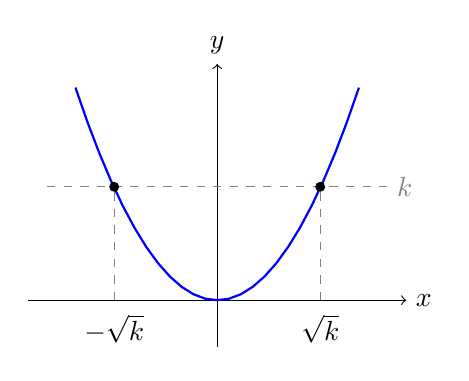
\begin{tikzpicture}[scale=1.2]
		\draw[->] (-2,0) -- (2,0) node[right] {$x$};
		\draw[->] (0,-0.5) -- (0,2.5) node[above] {$y$};
		\draw[thick, blue, domain=-1.5:1.5] plot (\x, {\x*\x});
		\draw[dashed, gray] (-1.8, 1.2) -- (1.8, 1.2) node[right] {$k$};
		\draw[dashed, gray] (1.09, 0) -- (1.09, 1.2);
		\draw[dashed, gray] (-1.09, 0) -- (-1.09, 1.2);
		\fill[black] (1.09, 1.2) circle (1.5pt);
		\fill[black] (-1.09, 1.2) circle (1.5pt);
		\node[below] at (1.09,-0.05) {$\sqrt{k}$};
		\node[below] at (-1.09,-0.05) {$-\sqrt{k}$};
	\end{tikzpicture}
\end{center}
